\section{Frontend}

Das Fronted der TeamDocument Applikation ist als React SPA entwickelt.
Einmal angemeldet kann ein Benutzer an der kollaborativen Bearbeitung des Dokumentes teilnehmen.

Folgende Interaktionen sind möglich:

\begin{itemize}
    \item Ändern des eigenen Namens
    \item Hinzufügen eines neuen Paragraphen
    \item Bearbeitung bestehender Paragraphen
    \item Sperren des Paragraphen an dem gerade gearbeitet wird (implizit)
    \item Verschieben von Paragraphen innerhalb des Dokuments
    \item Löschen eines bestehenden Paragraphen
    \item Wiederherstellen des zuletzt gelöschten Paragraphen (Hidden Feature)
\end{itemize}

Des Weiteren werden folgende Informationen auf dem UI dargestellt:

\begin{itemize}
    \item Name des ursprünglichen Autors eines Paragraphen
    \item Name des Autors welcher aktiv einen Paragraphen bearbeitet.
    \item Highlight des eigenen aktuellen Paragraphen
    \item Liste mit allen Dokumentupdates in chronologischer Reihenfolge
    \item Avatare aller aktiven Benutzer
\end{itemize}

\begin{figure}[H]
    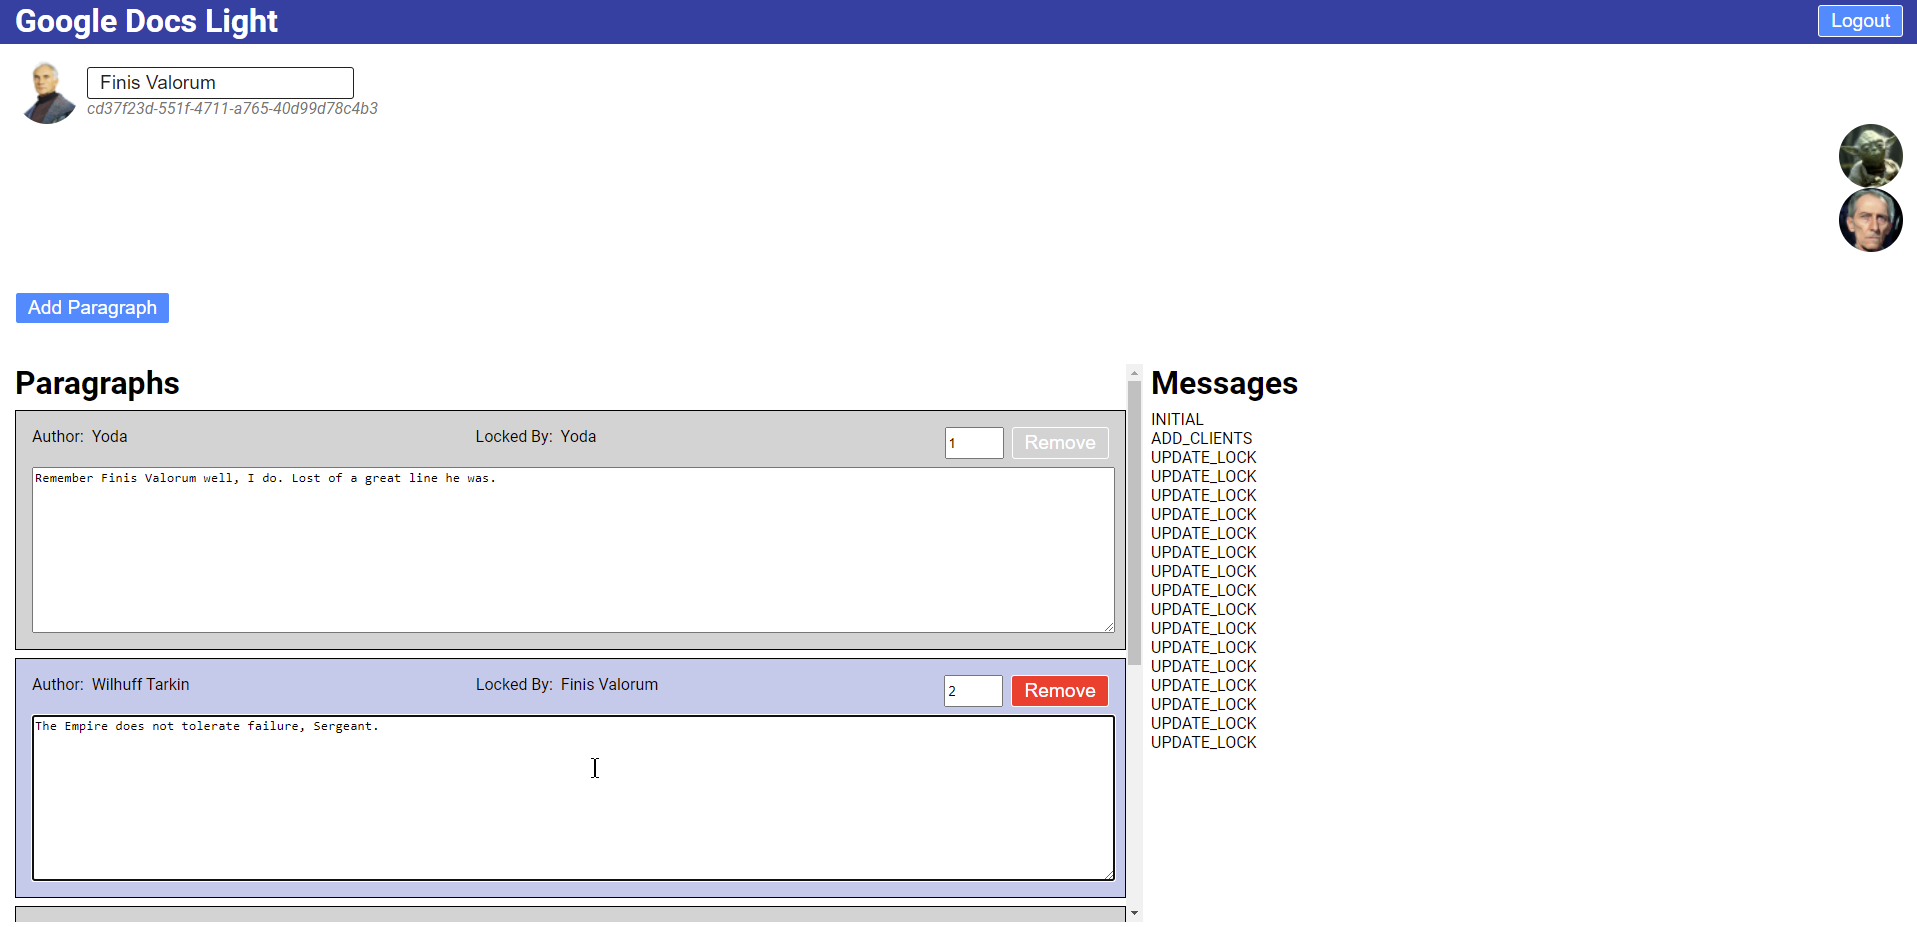
\includegraphics[width=\textwidth,keepaspectratio]{UI-blank}
    \caption{Team Document User Interface}
    \label{fig:Team Document User Interface}
\end{figure}


\subsection{Aufbau}

Die UI-Elemente sind als React-Komponenten umgesetzt und hierarchisch gegliedert.
Einzelne Komponenten nutzen zusätzliche Funktionalität, die in kleine Service Module ausgelagert ist.

Die Anbindung ans Backend ist mit zwei unidirektionalen Kanälen realisiert.

Der State der gesamten Applikation wird vom Redux Store bewirtschaftet.

\begin{figure}[H]
    \centering
    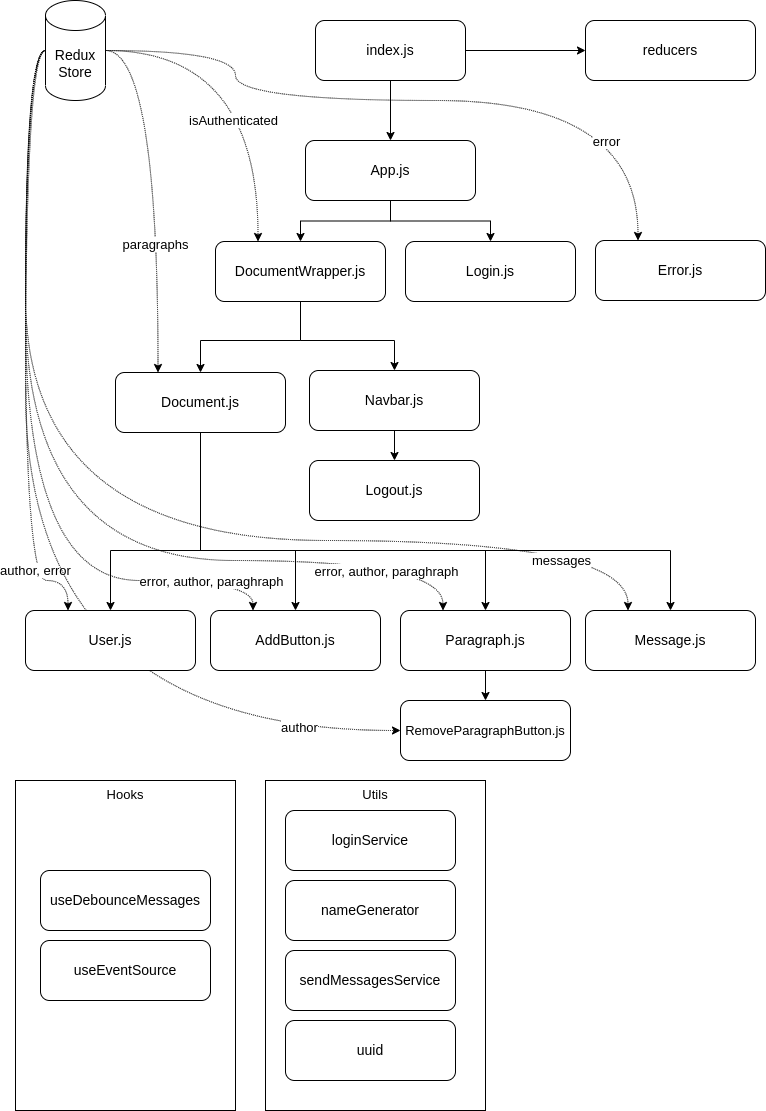
\includegraphics[width=\textwidth,keepaspectratio]{fe_structure}
    \caption{Komponenten Struktur}
    \label{fig: Fe_Structure}
\end{figure}

\subsubsection{Komponenten}

Alle Komponenten sind als Functional React Components implementiert.

\subsubsection*{index.js}
Das Index File ist der Eintrittspunkt für den Browser.
Beim Laden der Applikation wird der Redux Store erstellt und initialisiert.
Ebenfalls wird im Local Storage des Browsers geprüft, ob bereits ein User registriert ist.
Ist dies nicht der Fall, so wird ein zufälliger Benutzer generiert.

\subsubsection*{App.js}
Die App Komponente ist das äusserste Element, welches alle anderen Elemente hält.
Wir verwenden einen BrowserRouter um zwischen dem eigentlichen Dokument und der Login-Seite zu navigieren.

\subsubsection*{DocumentWrapper.js}
Wrapper um das Dokument zu schützen.
Solange sich ein User noch nicht ordentlich am Backend authentifiziert hat, leitet diese Komponente den Benutzer stetig auf die Login-Page weiter.

\subsubsection*{Login.js}
Login Formular, welches den Login Service verwendet.
Das Formular übersetzt die eingegebenen Credentials in einen Basic Auth Header und sendet damit einen GET Request ans Backend.
Bei erfolgreicher Authentifizierung wird das User Principal im Local Storage abgelegt.

\subsubsection*{Error.js}
Generische Fehlermeldung, welche als modales PopUp angezeigt wird, im Falle eines fehlgeschlagenen Requests.

\subsubsection*{Document.js}
Document repräsentiert den gesamten Zustand des Dokuments.
In dieser Komponente werden alle Paragraphen nach Position (Ordinal) sortiert aufgelistet.
Ebenfalls ist die Document Komponente der Parent für alle weiteren Elemente welche zum Dokument gehören.

\subsubsection*{Paragraph.js}
Die Repräsentation eines einzelnen Paragraphen.
Alle möglichen Änderungen eines einzelnen Paragraphen werden von dieser Komponente bewirtschaftet.


\subsubsection*{Message.js}
Message hält eine Liste aller verarbeiteten Commands, welche vom Backend empfangen wurden.

\subsubsection{Utils}
Im Ordner Utils sind Hilfsfunktionalitäten, welche von mehreren Komponenten verwendet werden oder nicht direkt einer Komponente zugehörig sind.

\subsubsection*{loginService.js}

\begin{itemize}
    \item login → Führt einen GET Request mit den übergebenen Credentials durch.
    \item logout → Entfernt das User Principal aus dem Local Storage
\end{itemize}

\subsubsection*{nameGenerator.js}

\begin{itemize}
    \item fetchSampleName → Abfrage bei https://akabab.github.io/starwars-api/api/id/ um einen zufälligen Autor zu erstellen
\end{itemize}

\subsubsection*{reducer.js}
Die eigentliche Fachlogik des Frontends ist im Reducer implementiert.
Alle Änderungen am Zustand des Dokuments werden von einer Funktion in der Function Map durchgeführt.
Die Funktionen entsprechen weitestgehend den Command Types beschrieben in Kapitel 4.5.
Zusätzlich werden vom Reducer noch der Authentifizierungszustand sowie ein Fehlerzustand gesetzt.

\subsubsection{Hooks}
Hooks erlauben React Features wie State oder andere Hooks zu verwenden, ohne das eine Klasse geschrieben wird.
Wir verwenden zwei Custom Hooks welche Funktionalität für mehrere Komponenten bereitstellen.

\subsubsection*{useEventSource.js}
Diese Hook erstellt beim erstmaligen Laden einer Komponente eine Referenz auf eine Polyfill Eventsource.
Diese ist die Schnittstelle auf welcher das Backend Updates veröffentlicht.

Die Polyfill Eventsource erlaubt im Gegensatz zum Browser-Default das HTTP-Header mit übergeben werden können.
Es gelten folgende Browser Kompatibilitäten

\begin{itemize}
    \item IE 10+, Firefox 3.5+, Chrome 3+, Safari 4+, Opera 12+
    \item IE 8 - IE 9: XDomainRequest is used internally, which has some limitations (2KB padding in the beginning is required, no way to send cookies, no way to use client certificates)
    \item It works on Mobile Safari, Opera Mobile, Chrome for Android, Firefox for Android
    \item It does not work on: Android Browser(requires 4 KB padding after every chunk), Opera Mini
\end{itemize}
\footnote{\url{https://github.com/Yaffle/EventSource#browser-support}}

\subsubsection*{useDebounceMessages.js}
Jedes einzelne Update innerhalb eines Paragraphen generiert einen POST-Request.
Es hat sich gezeigt das dieser Ansatz bei mehreren Benutzern, welche gleichzeitig schnell schreiben, einen Flaschenhals bildet.
In extremen Fällen haben sich einzelne Requests gegenseitig überholt.
Dadruch entstand für alle anderen Teilnehmer ein Flackereffekt in den entsprechenden Paragraphen.
Um die HTTP-Schnittstelle zu entlasten werden sämtliche Textupdates mit einem leichten Debounce aggregiert und so als Liste von einzeln Commands an der Server geschickt.
Das Debounce Delay ist auf 150 ms gesetzt.
Dementsprechend wird die Liste mit Updates erst nach einer Eingabepause von 150 ms versendet.
Je nach Tippgeschwindigkeit werden so zwischen 5 und 15 Commands aggregiert.
Dies hat zu einer signifikaten Entlastung der Netzwerklast geführt.

\begin{figure}[H]
    \centering
    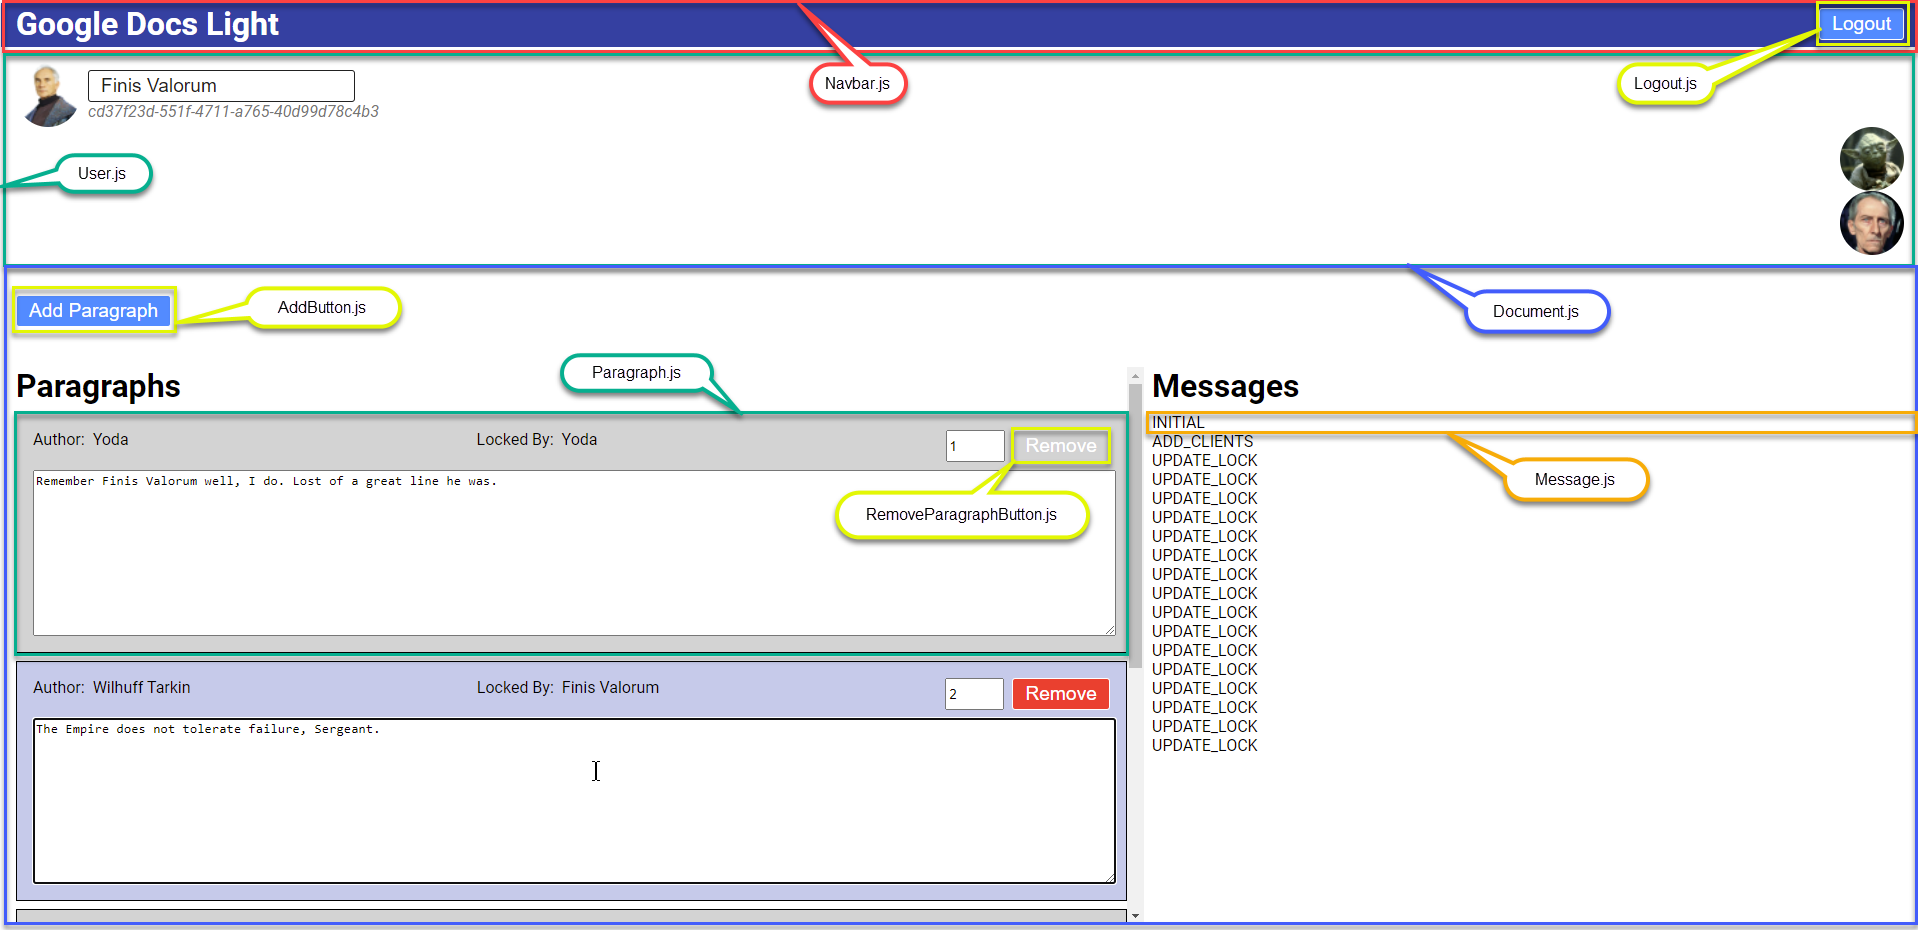
\includegraphics[width=\textwidth,keepaspectratio]{UI-components}
    \caption{UI-Components}
    \label{fig: UI-Components}
\end{figure}

\subsection{State- und Konfliktmanagment}
Der gesamte Zustand der Applikation ist im Redux Store abgebildet.
Der Zustand enthält folgende Komponenten:

\begin{tabbing}
    Left \= Middle \= Right \= Right \kill
    Key:  \> \> \> isAuthenticated\\
    Type:  \> \> \> Boolean \\
    Beschreibung \>  \> \> Flag für Routing zur Login-Page, falls false\\
\end{tabbing}

\begin{tabbing}
    Left \= Middle \= Right \= Right \kill
    Key:  \> \> \> author\\
    Type:  \> \> \> Object \{id: UUID, name: String, image: String\} \\
    Beschreibung \>  \> \> Repräsentation des eigenen Autors.\\
\end{tabbing}

\begin{tabbing}
    Left \= Middle \= Right \= Right \kill
    Key:  \> \> \> otherAuthors\\
    Type:  \> \> \> Array \\
    Beschreibung \>  \> \> Liste aller anderen aktiven Autoren.\\
\end{tabbing}

\begin{tabbing}
    Left \= Middle \= Right \= Right \kill
    Key:  \> \> \> paragraphs\\
    Type:  \> \> \> Array \\
    Beschreibung \>  \> \> Liste aller vorhandenen Paragraphen.\\
\end{tabbing}

\begin{tabbing}
    Left \= Middle \= Right \= Right \kill
    Key:  \> \> \> messages\\
    Type:  \> \> \> Array \\
    Beschreibung \>  \> \> Liste der vom Server erhaltenen Commands.\\
\end{tabbing}

\begin{tabbing}
    Left \= Middle \= Right \= Right \kill
    Key:  \> \> \> error\\
    Type:  \> \> \> Object\{isPresent: Boolean, message: String\} \\
    Beschreibung \>  \> \> Objekt welches einen Fehler anzeigt sofern einer vorhanden ist\\
\end{tabbing}

Beim Laden des Frontends baut der Client die Eventsource zum Server auf.
Dieser sendet anschliessend den aktuellen Zustand des Dokuments mit einem Initial Command zum Client.

Änderungen an der eigenen Kopie des Dokumentes werden direkt als Action an den Reducer dispatched.
Parallel wird die Änderung als Command an den Server gesendet welcher den Zustand des Dokuments aktualisiert und an alle anderen Teilnehmer weiterleitet.

Allfällige Konflikte werden dabei vom Server detektiert und aufgelöst.
Diese Korrekturen werden dann von allen Clients verarbeitet.

Das nachfolgende Ablaufdiagramm stellt die möglichen Varianten von Mutationen innerhalb des Frontends dar.

\begin{figure}[H]
    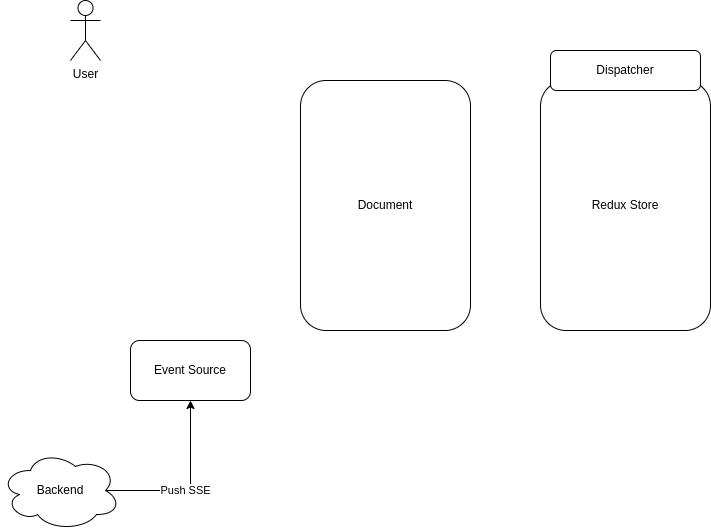
\includegraphics[width=0.9\textwidth,keepaspectratio]{fe_dataflow}
    \caption{Ablaufdiagramm}
\end{figure}

\subsection{Fehler Behandlung}
Fachliche Fehler werden vom Client nicht behandelt.
Möglich Fehler sind noch Verbindungsprobleme zum Server oder ungültige Zustände des Servers.

Ist der Server nicht erreichbar, wird das UI blockiert, sodass keine Eingaben mehr möglich sind.
Der Benutzer wird mit einer entsprechenden Fehlermeldung auf das Problem aufmerksam gemacht.

\begin{figure}[H]
    \centering
    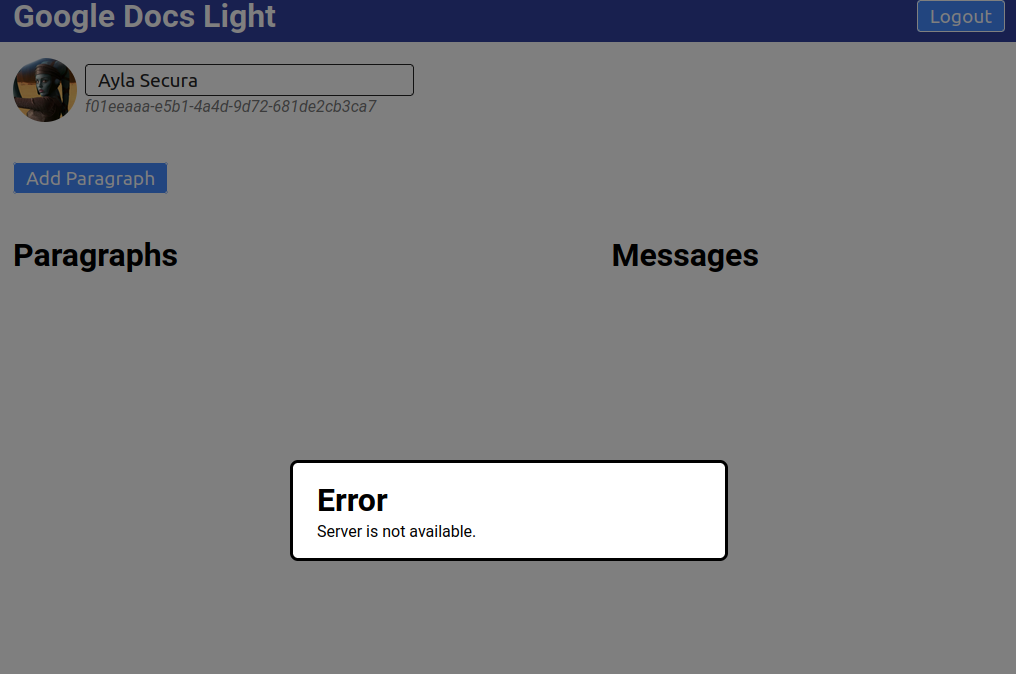
\includegraphics[width=\textwidth,keepaspectratio]{errormessage}
    \caption{Fehler Meldung}
\end{figure}

Beim Wiederherstellen der Verbindung zum Server wird von diesem der aktuelle Zustand des Dokumentes mit einem Initial-Command geladen.
